%%%% Time-stamp: <2012-08-20 17:41:39 vk>

%% example text content
%% scrartcl and scrreprt starts with section, subsection, subsubsection, ...
%% scrbook starts with part (optional), chapter, section, ...

\section{Annual Report}
\subsection{Overview}
JD.com, Inc’s Annual Report for FY 2016 comprises the mainly three parts:
\begin{enumerate}
	\item[\uppercase\expandafter{\romannumeral1}] This part includes corporate information, introducing the development of the company, the basic strategy, and brief operating and financial situation during the last year. It also includes the information about its directors, managers and employees. And also the strategy towards them is included.
	\item[\uppercase\expandafter{\romannumeral2}] This part introduces the details of the company’s dividend policy. It also includes the adjustments to statements and its principal of accounting.
	\item[\uppercase\expandafter{\romannumeral3}] The third part is mainly about JD’s financial statements and exhibits of materials.
	\item[\uppercase\expandafter{\romannumeral4}] This part is JD’s financial statements and its principal to record.
\end{enumerate}

JD.com, Inc. annual report for FY 2016 provides a detailed and comprehensive review of the operating and financial performance of the issuer of the annual report and its principal subsidiaries in the last financial year.

\subsection{External Users}
External users of the annual report include present and potential investors (equity owners), employees of the company, lenders of funds, customers, suppliers, government agencies and other members of the public: 
\begin{itemize}
\item \textbf{Investors.} The providers of risk capital and their advisers are concerned with the risk inherent in, and return provided by, their investments.  They need information to help them determine whether they should buy, hold or sell.  Shareholders are also interested in information that enables them to assess the ability of the enterprise to pay dividends. 
\item \textbf{Employees.} Employees and their representative groups are interested in information about the stability and profitability of their employers.  They are also interested in information which enables them to assess the ability of the enterprise to provide remuneration, retirement benefits and employment opportunities. 
\item \textbf{Lenders.} Lenders are interested in information that enables them to determine whether their loans, and the interest attaching to them, will be paid when due. 
\item \textbf{Suppliers and other trade creditors.} Suppliers and other creditors are interested in information that enables them to determine whether amounts owing to them will be paid when due. Trade creditors are likely to be interested in an enterprise over a shorter period than lenders unless they are dependent upon the continuation of the enterprise as a major customer. 
\item \textbf{Customers.} Customers have an interest in information about the continuance of an enterprise, especially when they have a long-term involvement with, or are dependent on, the enterprise. 
\item \textbf{Governments and their agencies.} Governments and their agencies are interested in the allocation of resources and, therefore, the activities of enterprises.  They also require information in order to regulate the activities of enterprises, determine taxation policies and as the basis for national income and similar statistics. 
\item \textbf{Public.} Enterprises affect members of the public in a variety of ways.  For example, enterprises may make a substantial contribution to the local economy in many ways including the number of people they employ and their patronage of local suppliers.  Financial statements may assist the public by providing information about the trends and recent developments in the prosperity of the enterprise and the range of its activities.
\end{itemize}
While the objective of annual reports is to provide information about the financial position, performance and changes in financial position of an enterprise, it cannot cater to all the information needs of users. However, as investors are providers of risk capital to the enterprise, financial information from the annual report that meet their needs will also meet the common needs of other users.

\section{Corporate Governance}
\subsection{Board of Directors}

\begin{table}[H]	
\begin{center}
\begin{tabular}{ l|l }
	\hline
	\multicolumn{2}{c}{\textbf{Board of Directors}} \\
	\hline
	Richard Qiangdong Liu	&		Chairman and Chief Executive Officer \\
	\rowcolor[gray]{.95}
	Martin Chiping Lau		& 		Director\\
	Ming Huang				&		Independent Director \\
	\rowcolor[gray]{.95}
	Louis T. Hsieh			&		Independent Director \\
	David Daokui Li			&		Independent Director \\
	\hline
\end{tabular}
\end{center}
\caption{Board of directors of JD.com, Inc}\label{table:1}
\end{table}


	
 
\subsubsection{Appointment of New Directors}
\subsubsection{Directors’ Remuneration}
In 2016, JD paid an aggregate of approximately RMB12.7 million (US\$1.8 million) in cash to their executive officers, and approximately US\$0.2 million in cash to their non-executive directors. They have not set aside or accrued any amount to provide pension, retirement or other similar benefits to their executive officers and directors\footnote{See JD.com, Inc. annual report 2016, Page 115}.
The details of remuneration are not mentioned in the report.

\subsubsection{Directors’ Appointments in Other Institutions}
Martin Chiping Lau is the only director who also holds positions in other institutions.
The situation is as follows:

\begin{table}[H]	
	\begin{center}
		\begin{tabular}{ |l|l|l| }
			\hline
			\rowcolor[gray]{.95}
			\textbf{DIRECTOR}	& \textbf{COMPANY} &\textbf{APPOINTMENT} \\
			\hline
			 	            	& Tencent Holdings Limited & President and Executive Director\\			 	            	
			Martin Chiping Lau	& Leju Holdings Limited & Director \\
			 			        & Kingsoft Corporation Limited &Non-Executive Director \\
			\hline
		\end{tabular}
	\end{center}
	\caption{Directors’ Appointments in Other Institutions}\label{table:1}
\end{table}

\subsubsection{Directors’ Interests in Shares and Debentures}
The following table sets forth information with respect to the beneficial ownership of our ordinary shares as of February 28, 2017 by\footnote{See JD.com, Inc. annual report 2016, Page 122}:
\begin{itemize}
	\item each of our directors and executive officers; and
	\item each person known to us to own beneficially more than 5\% of our total outstanding shares.
\end{itemize}

\begin{table}[H]	
	\begin{center}
		\begin{tabular}{|l|p{2.05cm}|c|p{2.05cm}|c|c}\hline
			        &\multicolumn{2}{c|}{DIRECT INTEREST}&\multicolumn{2}{c|}{DEEM INTEREST}\\
			        \hline
			Director&Beginning of Year&End of Year&Beginning of Year&End of Year\\
			\hline
			Richard Qiangdong Liu&452,044,989&452,044,989& &\\
			\hline
		\end{tabular}
	\end{center}
	\caption{Board of directors of JD.com, Inc}\label{table:1}
\end{table}

\subsubsection{Share Options}
A director is not required to hold any shares in JD’s company by way of qualification. A director who is in any way, whether directly or indirectly, interested in a contract or transaction or proposed contract or transaction with the company must declare the nature of his interest at a meeting of the directors.

Under JD’s current memorandum and articles of association, our board of directors will not be able to form a quorum without Mr. Richard Qiangdong Liu for so long as Mr. Liu remains a director\footnote{See JD.com, Inc. annual report 2016, Page 118}.

\subsection{Audit Committee}
JD’s audit committee consists of Louis T. Hsieh, Ming Huang and David Daokui Li. Mr. Hsieh is the chairman of their audit committee.
The audit committee oversees JD’s accounting and financial reporting processes and the audits of the financial statements of our company.
The audit committee is responsible for, among other things:
\begin{itemize}
\item Appointing the independent auditors and pre-approving all auditing and non-auditing services permitted to be performed by the independent auditors;
\item Reviewing with the independent auditors any audit problems or difficulties and management’s response;
\item Discussing the annual audited financial statements with management and the independent auditors;
\item Reviewing the adequacy and effectiveness of our accounting and internal control policies and procedures and any steps taken to monitor and control major financial risk exposures;
\item Reviewing and approving all proposed related party transactions;
\item Meeting separately and periodically with management and the independent auditors;
\item Monitoring compliance with our code of business conduct and ethics, including reviewing the adequacy and effectiveness of our procedures to ensure proper compliance.
\end{itemize}

\subsection{Nominating and Corporate Governance Committee}
JD’s nominating and corporate governance committee consists of David Daokui Li and Louis T. Hsieh. Mr. Li is the chairperson of their nominating and corporate governance committee. The nominating and corporate governance committee is responsible for, among other things:
\begin{itemize}
\item	Selecting and recommending to the board nominees for election by the shareholders or appointment by the board;
\item	Reviewing annually with the board the current composition of the board with regards to characteristics such as independence, knowledge, skills, experience and diversity;
\item	Making recommendations on the frequency and structure of board meetings and monitoring the functioning of the committees of the board;
\item	Advising the board periodically with regards to significant developments in the law and practice of corporate governance as well as our compliance with applicable laws and regulations, and making recommendations to the board on all matters of corporate governance and on any remedial action to be taken.
\end{itemize}

\subsection{Internal Control}
Internal control assists in the company’s effective and efficient operations by helping it to react suitably to significant business, operational, financial, compliance and other risks to achieve the company’s aims. JD did not employ any internal auditors.


\subsection{Independent Auditors}
Mr. Hsieh, Mr. Huang and Mr. Li in the company’s audit committee satisfy the “independence” requirements of NASDAQ and Rule 10A-3 under the Securities Exchange Act of 1934. It provides service as states in 3.1.



\section{Operating Activities}
The principal activities of the Company are online direct sales, online marketplace and other services. Its subsidiaries are principally set to assistant their operating activities, all of which were built in China.
The Company comprises the following branches and subsidiaries:
\begin{itemize}
\item Jingdong Century-Established in April 2007, and certain of its subsidiaries in China, which primarily engage in retail business;
\item	Shanghai Shengdayuan Information Technology Co., Ltd., or Shanghai Shengdayuan-Established in April 2011 and primarily operates their online marketplace business;
\item	Tianjin Star East Corporation Limited, or Star East-Established in April 2012 and provides primarily warehousing and related services;
\item	Beijing Jingbangda Trade Co., Ltd., or Jingbangda-Established in August 2012 and provides primarily courier services.
\end{itemize}

The success of this company hinges on their ability to provide superior customer experience. Their slogan is “selection, speed, quality, value”, and they are committed to optimizing customer experience and achieving customer satisfaction. They rely on online direct sale of computer, communication and consumer electronics for a significant portion of their net revenues.

The director of the Group admitted that they have incurred significant net losses and they may continue to experience significant losses in the future. It is also reported that if they are unable to provide superior customer experience, their business and reputation may be materially and adversely affected.

JD plan to further expand their fulfillment infrastructure. If they are not able to manage such expansion successfully, their growth potential, business and results of operations may be materially and adversely affected.

Cost of revenue account for the Group’s most cost and expense, and it decrease by 1.8\% during 2016. Fulfillment increases by 0.4\%, technology and content increases by 0.3\% and general and administrative increases by 0.2\%. While marketing decreases 0.2\% and impairment of goodwill and intangible assets decreases 1.5\%. This decrease in expense more than offset the increase in expense which resulted in loss decrease of 3.7\% as a percentage of revenue.

\section{Income Statement}

The Group’s income statement covers the period from 1 January 2014 to 31 December 2016.

Turnover represents online direct sales, services and others. The Group’s turnover is as follows:
\begin{table}[H]	
	\begin{center}
		\begin{tabular}{lcccc}
			\toprule
			 &\textbf{2015}&\textbf{2016}&\textbf{Absolute change}&\textbf{Ralative change}\\
			 
			\midrule
	    	Turnover&181,275&260,122&78,847&43.5\%\\
			\bottomrule
		\end{tabular}
	\end{center}
	\caption{Turnover (in thousands of RMB \textyen)}\label{table:1}
\end{table}

The increase of 43.5\% in turnover from FY 2015 was achieved from an increase in online direct sales, which dominants about 38.6\%.

\subsection{Group Revenue According to Activities}

\begin{table}[H]	
	\begin{center}
		\begin{tabular}{lrr}
			\toprule
			&\textbf{2015}&\textbf{2016}\\
			\midrule
		    Online direct sales&167,721&237,702\\
			Services and others&13,554&22,420\\
			\qquad\emph{Total}&181,275&260,122\\
			\bottomrule
		\end{tabular}
	\end{center}
	\caption{Revenue (in thousands of RMB \textyen)}\label{table:1}
\end{table}

The Group’s online direct sales increases 41\% and services an others increase 65\%, resulting in 38.6\% increase in turnover. This illustrates a good state of operation during year 2016. We can also calculate that online direct sales generates the most profit for the company.

\subsection{Revenue Recognition}

The Group recognizes revenues from advertising placements ratably over the period during which the advertising services are provided or on the number of times that the advertisement has been displayed based on cost per thousand impressions, and recognizes revenues from pay for performance marketing services based on effective clicks.

The Group offers consumer financing to individual customers and supply chain financing to suppliers and merchants on the Group’s online marketplace. Revenues resulting from these financing services are recognized in accordance with the contractual terms.

The Group recognizes the revenues from the online direct sales on a gross basis as the Group is primarily obligated in these transactions, is subject to inventory risk, has latitude in establishing prices and selecting suppliers, or has met several but not all of these indicators.

The Group earns transaction fees from processing transactions for online payment customers. Services resulting from these transactions are recognized as service revenues when processing services are completed.

Advertising arrangements involving multiple deliverables are allocated into single-element arrangements based on their relative selling price in the absence of both vendor specific objective evidence and third party evidence, and the related revenue is recognized over the period during which the element is provided.

\subsection{Common Size Income Statement}
The Common Size Income Statement is as follows:

\begin{table}[H]	
	\begin{center}
		\begin{tabular}{lrrr}
			\toprule
			&\textbf{2015}&\textbf{2016}&\textbf{Change}\\
			\midrule
			Net revenues&	100&	100&	-\\
			Cost and Expenses& & & \\			
			Cost of revenues&	86.6&	84.8&	(1.8)\\
			Fulfillment&7.7&	8.1	&	0.4\\
			Marketing&	4.3&	4.1	&(0.2)\\
			Technology and content&	1.8&	2.1&	0.3\\
			General and administrative&	1.6	&1.8&	0.2\\
			Impairment of goodwill and intangible assets&	1.5&0&	(1.5)\\
			Other expense&1.5&	0.4	&	(1.1)\\
			Total costs and expenses&	105.0&	101.3&	(3.7)\\
			Loss before taxation&5.0&	1.3	&	(3.7)\\
			Taxation&	(0.007)&	0.008&	0.015\\
			Loss for Year	&5.0&	1.3&	(3.7)\\
			\bottomrule
		\end{tabular}
	\end{center}
	\caption{Common Size Income Statement (in percents)}\label{table:1}
\end{table}

Cost of revenue account for the Group’s most cost and expense, and it decrease by 1.8\% during 2016. Fulfillment increases by 0.4\%, technology and content increases by 0.3\% and general and administrative increases by 0.2\%. While marketing decreases 0.2\% and impairment of goodwill and intangible assets decreases 1.5\%. This decrease in expense more than offset the increase in expense which resulted in loss decrease of 3.7\% as a percentage of revenue.


\subsection{Net Loss Before Tax}
The Net Income before tax is as follows:

\begin{table}[H]	
	\begin{center}
		\begin{tabular}{lcccc}
			\toprule
			&\textbf{2015}&\textbf{2016}&\textbf{Absolute change}&\textbf{Ralative change}\\
			
			\midrule
			Net loss before tax&9,132&3,234&(5898)&(64.6\%)\\
			\bottomrule
		\end{tabular}
	\end{center}
	\caption{Net loss before tax (in thousands of RMB \textyen)}\label{table:1}
\end{table}

The loss of the Group decreased by an approximate RMB 5,898,000. The percentage  decrease was 64.6, mainly resulting from decreases in operating expenses especially cost of revenue.

\subsection{Retained Earnings }

The retained earnings are as follows:

\begin{table}[H]	
	\begin{center}
		\begin{tabular}{lrrr}
			\toprule
			&\textbf{2015}&\textbf{2016}\\
			\midrule
			Balance at 1 January&	15,009&	55,560\\
			Statutory reserves&	40,551&	77,378\\
			Balance at 31 December&	55,560&	132,938\\
			\bottomrule
		\end{tabular}
	\end{center}
	\caption{Retained earnings (in thousands of RMB \textyen)}\label{table:1}
\end{table}

The Group’s retained earnings largely increased during year 2015 and 2016. Statutory reserves every year also had a large increase, which indicated full cash flow of the company.

\subsection{Earnings Per Share}
	The Earnings per share is as follows:
\begin{table}[H]	
	\begin{center}
		\begin{tabular}{lccc}
			\toprule
			&\textbf{2015}&\textbf{2016}&\textbf{Change}\\
			\midrule
			Basic and diluted earnings per share&(3.33) cents&(1.36) cents&148.12\%\\
			\bottomrule
		\end{tabular}
	\end{center}
	\caption{Earnings per share}\label{table:1}
\end{table}

Earnings per share of the Group was negative due to a negative profit of the company. However, a positive change of it shows that the Group has an improvement in profit.

\section{Taxes}
\subsection{Taxation Summary}

The Group is imposed on the following three sorts of taxes\footnote{See JD.com, Inc. annual report 2016, Page F-53}:
\begin{itemize}
	\item \textbf{Value added tax.}
    During the periods presented, the Group is subject to statutory VAT\footnote{A pilot program for transition from business tax to value added tax (“VAT”) for certain services revenues was launched in Shanghai on January 1, 2012.} rate of 13\% and 17\% for revenues from sales of audio, video products and books and sales of other products, respectively, in the PRC. 
	\item \textbf{Business tax.}
	Before May 1, 2016, the Group was subject to 5\% business tax and related surcharges for revenues from online payment services. Starting from May 1, 2016, the Group is subject to 6\% VAT for revenues from online payment	services. Business tax and the related surcharges are recognized when the revenue is earned.
	\item \textbf{Income tax.}
	Three subsidiaries of the Group, Beijing Shangke, Chongqing Haijia and Chengdu Century, enjoyed a preferential
	income tax rate of 15\%. The Group’s other PRC subsidiaries, VIEs\footnote{A variable interest entity (VIE) is an entity that an investor has a controlling interest in, but this controlling interest is not based on a majority of voting rights.} and VIEs’ subsidiaries are subject to the statutory income tax rate of 25\%. 
\end{itemize}
As a  matter of fact, JD.com attempts to obtain tax allowance and exemption by being classified as “high and new technology enterprises”. 
\subsection{Income Tax}

The Group follows the liability method of accounting for income taxes\footnote{See JD.com, Inc. annual report 2016, Page F-30}. Under this method, deferred tax assets and liabilities are determined based on the temporary differences between the financial statements carrying amounts and tax bases of existing assets and liabilities by applying enacted statutory tax rates that will be in effect in the period in which the temporary differences are expected to reverse. 

The amounts of income tax benefits or expenses for the year ended December 31, 2015 and the year ended December 31,2016 are tabulated as follows\footnote{See JD.com, Inc. annual report 2016, Page F-55}:

\begin{table}[H]	
	\begin{center}
		\begin{tabular}{lcc}
			\toprule
			&\textbf{2015}&\textbf{2016}\\
			\midrule
			Current income tax expenses&(28,322)&(214,282)\\
			Deferred tax benefits&\underline{42,584}&\underline{34,782}\\
			\qquad\emph{Income tax benefits/(expenses)}&\uuline{14,262}&\uuline{(179,500)}\\
			\bottomrule
		\end{tabular}
	\end{center}
	\caption{Income tax benefits or expenses (in thousands of RMB \textyen)}\label{table:1}
\end{table}


It is noteworthy that the Group reports income tax benefits rather than income tax expenses for the fiscal year 2015. The result is caused by its considerable deferred tax benefits which amounts to the increase in deferred tax assets less the decrease in deferred tax liabilities. In accordance with the regulations of the relevant tax jurisdictions, the Group's net operating loss generates deferred tax assets which may be used to deduct the income tax incurred in the next five fiscal years, if the Group can make a profit in the foreseeable future.

With the Group's net loss decreasing year by year, we can expect income tax expenses rather than tax benefits to be reported. 

\section{Dividends}
\subsection{Factors on Dividend Policy}
There are several factors that influence whether a company pays a dividend and how much it chooses to pay. Some of the most influential factors are listed as follows.
\begin{itemize}
	\item \textbf{Income stability.} 
	Income stability is one of the top factors in determining dividend policies. Specifically, established companies with stable, predictable income streams are more likely to pay dividends than companies with growing or volatile income.\\
	Newer and rapidly growing companies rarely pay dividends, as they prefer to invest their profits back into the company to fuel even more future growth. And, companies with unstable revenue streams often choose not to pay dividends, or pay small dividends in order to make sure the payout will be sustainable.\\
	It looks terrible to investors when companies are forced to suspend or reduce dividend payments, so most like to err on the side of caution when deciding to implement a new dividend, waiting for several years of stable profits before doing so.	
	
	\item  \textbf{Profitability.}
	Another factor that can influence management's dividend policies is the potential for better returns through capital reinvestment. In other words, if a company feels that it would be in the best interest of its shareholders to use its profits for other business activities besides paying dividends, it could choose not to pay – even if its revenues are stable and predictable.\\
	One great example of this is Warren Buffett's Berkshire Hathaway, which has never paid a dividend. Instead, Buffett feels that reinvesting the company's profits is a far better idea -- and he's been right. Berkshire has produced phenomenal returns for decades, and a big reason was the compounding effect of reinvesting its profits instead of paying them out.
	
	\item \textbf{Taxes.}
	Dividends are effectively taxed twice -- once at the corporate level, and again when they are paid out to shareholders.\\
	Because of this, many companies (and their investors) feel that other methods of returning capital, such as share repurchases, are a better way to go. Repurchasing shares has the same net effect as a dividend payment -- the intrinsic value of the company's shares increases as the share count drops. However, this can allow investors who like to reinvest their dividends to do so without having to worry about dividend taxes.
	
	\item \textbf{Legal requirements.} 
	It's also worth noting that some companies have no choice but to pay dividends. For example, real estate investment trusts receive some pretty nice tax benefits, but they are legally required to pay at least 90\% of their income to shareholders.\\
	On the other hand, some companies need to obtain approval before paying or increasing their dividends. Since the financial crisis, many banks need to submit capital plans for regulatory approval for any plans to boost their payouts.
	
	\item \textbf{Economic conditions.}
	Finally, another major factor that influences dividend policies is the market environment. If a certain sector is having trouble and anticipates profits falling, it's common for companies to get quite defensive when it comes to their dividends.\\	
	This can be seen currently in the energy sector, where low oil prices have wreaked havoc on many companies' profitability, which has led to several major companies slashing their dividends recently.
\end{itemize}

As for JD.com, Inc., it stated that the form, frequency and amount of dividend payment will depend upon its future operations and earnings, capital requirements and surplus, general financial condition, contractual restrictions and other factors that the board of directors may deem\footnote{See JD.com, Inc. annual report 2016, Page 130}.


\subsection{Dividend Policy Performed by the Group}
JD.com, Inc. does not reflect an active attitudes towards dividend payment. So far the Group have not declared or paid any dividends on ordinary shares, nor it have any present plan to pay any cash dividends on ordinary shares in the foreseeable future\footnote{See JD.com, Inc. annual report 2016, Page 131}. In the light of its heavy financial losses, it is not surprising that the Group Chose not to grant any dividends. The reason why stockholders are willing to purchase and hold the Group's stocks is unlikely for possible dividends. Instead, they may value its dominant position in electronic commerce and look ahead its future development with an optimistic expectation.


\section{Share Capital and Reserves}

\subsection{Share capital}

JD.com, Inc. holds outstanding shares consisting of ordinary shares, series A and A-1 convertible preferred shares and series B convertible preferred sharesas of December 31, 2013\footnote{See JD.com, Inc. annual report 2016, Page F-10}. Since 2014, the Group only has one class of shares, which is the Ordinary shares.

\renewcommand{\arraystretch}{0.83}
\begin{table}[H]	
	\begin{center}
		\begin{tabular}{p{5.6cm}rrrr}
			\toprule 
			& \multicolumn{2}{c}{\textbf{Ordinary shares}} & \multicolumn{2}{c}{\textbf{Treasury stock}} \\\cmidrule(lr){2-3} \cmidrule(lr){4-5} 
			\multirow{-2}{*}{} &\multicolumn{1}{c}{Shares}&Amount&\multicolumn{1}{c}{Shares}&\multicolumn{1}{c}{Amount}\\
		\midrule
		\rowcolor[gray]{.96}	
		Balance as of
		December 31,
		2015&2,793,756,650&358&(51,766,164)&(3)\\
		Issuance of ordinary shares&144,952,250&19&-&-\\
		\rowcolor[gray]{.96}
		Surrender of ordinary shares by certain	shareholder&(1)&-&-&-\\
		Exercise of sharebased	awards&-&-&2,820,648&77,496\\
		\rowcolor[gray]{.96}
		Share-based	compensation and vesting of sharebased	awards&-&-&8,812,582&78,903\\
		Balance as of December 31, 2016&2,938,708,899&377&(102,264,502)&(5,181,880)\\
		\bottomrule
		\end{tabular}
	\end{center}
	\caption{Share capital (amounts in thousands of RMB \textyen, shares in one)}\label{table:1}
\end{table}


\subsection{Bonus Issue}
A bonus issue, also known as a scrip issue or a capitalization issue, is an offer of free additional shares to existing shareholders. A company may decide to distribute further shares as an alternative to increasing the dividend payout. For example, a company may give one bonus share for every five shares held.

Companies give away bonus shares to shareholders when companies are short of cash and shareholders expect a regular income. Shareholders may sell the bonus shares and meet their liquidity needs. Bonus shares may also be issued to restructure company reserves. Issuing bonus shares does not involve cash flow. It increases the company’s share capital but not its net assets.


\subsection{Stock Split}
A stock split is a corporate action in which a company divides its existing shares into multiple shares to boost the liquidity of the shares. Although the number of shares outstanding increases by a specific multiple, the total dollar value of the shares remains the same compared to pre-split amounts, because the split does not add any real value. The most common split ratios are 2-for-1 or 3-for-1, which means that the stockholder will have two or three shares, respectively, for every share held earlier.

A stock split is also known as a forward stock split. In the UK, a stock split is referred to as a scrip issue, bonus issue, capitalization issue, or free issue.


\subsection{Rights Issue}
A rights issue is a dividend of subscription rights to buy additional securities in a company made to the company's existing security holders. When the rights are for equity securities, such as shares, in a public company, it is a non-dilutive pro rata way to raise capital. Rights issues are typically sold via a prospectus or prospectus supplement. With the issued rights, existing security-holders have the privilege to buy a specified number of new securities from the issuer at a specified price within a subscription period. In a public company, a rights issue is a form of public offering (different from most other types of public offering, where shares are issued to the general public).

Rights issues may be particularly useful for all publicly traded companies as opposed to other more dilutive financing options. As equity issues are generally preferable to debt issues from the company's viewpoint, companies usually opt for a rights issue in order to minimize dilution and maximize the useful life of tax loss carry forwards. Since in a rights offering there is no change of control and a "no-sale theory" applies, companies are able to preserve tax loss carry-forwards better than via either follow-on offerings or other more dilutive financings. It's one of the types in modes of issue of securities both in public and private companies.

\section{Current Assets and Current Liabilities}
\subsection{Current Assets}
A current asset is any asset which can reasonably be expected to be sold, consumed, or exhausted through the normal operations of a business within the current fiscal year. JD.com records 11 current assets accounts in its consolidated balance Sheet\footnote{See JD.com, Inc. annual report 2016, Page F-3}. 

We extract the following breakdown from JD.com, Inc. consolidated balance Sheet as of December 31, 2015 and as of December 31, 2016.\\

\begin{table}[H]	
\begin{center}
	\begin{tabular}{lrr}
		\toprule
		&\textbf{2015}&\textbf{2016}\\
		\midrule
		Cash and cash equivalents&17,863,868&19,771,695\\
		Restricted cash&2,114,913&4,391,955\\
		Short-term investments&2,780,482&4,391,955\\
		Investment securities&-&723,449\\
		Accounts receivable, net&8,193,665&17,464,408\\
		Advance to suppliers&927,177&1,423,736\\
		Inventories, net&20,539,543&28,909,438\\
		Loan receivables, net&3,698,488&12,697,915\\
		Other investments&-&10,766,920\\
		Prepayments and other current assets&1,486,441&2,198,906\\
		Amount due from related parties&\underline{863,516}&\underline{1,410,050}\\
		\qquad\emph{Total current assets}&\uuline{58,468,093}&\uuline{106,932,098}\\
		\bottomrule
	\end{tabular}
\end{center}
	\caption{Current assets (in thousands of RMB \textyen)}\label{table:1}
\end{table}
As we can see, the current assets jumped from \textyen58,468,093,000 to \textyen106,932,098,000. The total current assets increased substantially by 82.89\% in fiscal year 2016 as compared to fiscal year 2015. The item other investments accounts for a great portion of the increase. The Group invests in marketable equity securities to meet business objectives. These marketable securities are reported at fair value, classified and
accounted for as available-for-sale securities in investment securities.

Other investments represent the higher yield investments purchased by JD Finance and resold to third-party investors. JD Finance will earn yield
differentials. As JD Finance takes the majority risks and rewards of the products sold to the third-party investors, the Group reported the investments
purchased and the funds raised by sale of the financial products on a gross basis on the Consolidated Balance Sheets. 

In December 2014, the Group acquired 6.5\% equity interest in Tuniu with cash consideration of RMB305,930 (“Initial Investment”). Tuniu is a leading
online leisure travel company in China that is listed on the Nasdaq. The Group accounted for the Initial Investment as an available-for-sale security\footnote{See JD.com, Inc. annual report 2016, Page F 41}.

\subsection{Current Liabilities}

We extract the following breakdown from JD.com, Inc. consolidated balance Sheet.\\
 
\begin{table}[H]	
	\begin{center}
		\begin{tabular}{lrr}
			\toprule
			&\textbf{2015}&\textbf{2016}\\
			\midrule
			Short-term borrowings&3,040,209&8,333,317\\
			Nonrecourse securitization debt&579,843&9,389,213\\
			Accounts payable&29,819,341&4,391,955\\
			Advance from customers&7,173,885&43,988,087\\
			Deferred revenues&983,721&11,632,766\\
			Taxes payable&103,211&1,221,865\\
			Amount due to related parties&104,726&575,848\\
			Accrued expenses and other current liabilities&\underline{7,178,065}&\underline{167,655}\\
			\qquad\emph{Total current liabilities}&\uuline{48,983,001}&\uuline{104,740,235}\\
			\bottomrule
		\end{tabular}
	\end{center}
	\caption{Current liabilities (In thousands of RMB \textyen)}\label{table:1}
\end{table}

It indicates that the current liabilities jumped from \textyen48,983,001,000 to \textyen104,740,235,000. Current liabilities increased by 113.83\%. It is mainly because of a a sharp rise in Advance from customers.
	
\subsection{Working Capital}
The working capital of the Group is tabulated as follows:
\begin{table}[H]	
	\begin{center}
		\begin{tabular}{lrrr}
			\toprule
			&\textbf{2015}&\textbf{2016}&\textbf{Change}\\
			\midrule
			Working capital&9,485,092&2,191,863&(76.89\%)\\
			\bottomrule
		\end{tabular}
	\end{center}
	\caption{Working capital (In thousands of RMB \textyen)}\label{table:1}
\end{table}

Working capital is a measure of a company’s efficiency and short-term financial health. The 76.89\% decrease in working capital in fiscal year 2016 signifies underling problem on healthier liquidity.

\subsection{Current Ratio}
The Current ratio of the Group is tabulated as follows:
\begin{table}[H]	
	\begin{center}
		\begin{tabular}{lrrr}
			\toprule
			&\textbf{2015}&\textbf{2016}&\textbf{Change}\\
			\midrule
			Current ratio&1.194&1.021&14.49\%\\
			\bottomrule
		\end{tabular}
	\end{center}
	\caption{Current ratio}\label{table:1}
\end{table}

The current ratio is a liquidity ratio that measures a company's ability to pay short-term and long-term obligations. To gauge this ability, the current ratio considers the current total assets of a company (both liquid and illiquid) relative to that company’s current total liabilities. 

The decreasing current ratio also implies that the Group are under pressure to pay the creditor back. Some potential creditors may doubt whether the Group in question would be able to pay off its obligations if they came due at that point. 



\subsection{Quick Ratio}
\begin{table}[H]	
	\begin{center}
		\begin{tabular}{lrr}
			\toprule
			&\textbf{2015}&\textbf{2016}\\
			\midrule
			Quick ratio&(37.46\%)&(25.51\%)\\
			\bottomrule
		\end{tabular}
	\end{center}
	\caption{Quick ratio}\label{table:1}
\end{table}
The quick ratio reflects the ability of a company to repay its short-term obligations with its more liquid assets. 


\section{Inventories}
\subsection{Inventory Values}

Inventories, net, consist of the following\footnote{See JD.com, Inc. annual report 2016, Page F-48}:
\begin{table}[H]	
	\begin{center}
		\begin{tabular}{lrr}
			\toprule
			&\textbf{2015}&\textbf{2016}\\
			\midrule
			Products&20,436,275&28,778,528\\
			Packing materials and others&\underline{103,268}&\underline{130,910}\\
			\qquad\emph{Inventories, net}&\uuline{20,539,543}&\uuline{28,909,438}\\
			\bottomrule
		\end{tabular}
	\end{center}
	\caption{Inventories, net (in thousands of RMB \textyen)}\label{table:1}
\end{table}

\subsection{Inventory Valuation Policy}
Inventories, consisting of products available for sale, are stated at the lower of cost or market value\footnote{See JD.com, Inc. annual report 2016, Page F-20}. Cost of inventory is determined using the weighted
average cost method. Adjustments are recorded to write down the cost of inventory to the estimated market value due to slow-moving merchandise and
damaged goods, which is dependent upon factors such as historical and forecasted consumer demand, and promotional environment. The Group takes
ownership, risks and rewards of the products purchased, but has arrangements to return unsold goods with certain vendors. Write downs are recorded in cost of
revenues in the Consolidated Statements of Operations and Comprehensive Loss.

The Group also provides fulfillment-related services in connection with the Group’s online marketplace. Third-party sellers maintain ownership of their
inventories and therefore these products are not included in the Group’s inventories.
\subsection{Gross Profit Percentage on Sale}

The gross profit ratio is important because it shows management and investors how profitable the core business activities are without taking into consideration the indirect costs. This gives investors a key insight into how healthy the company actually is. For instance, a company with a seemingly healthy net income on the bottom line could actually be dying. The gross profit percentage could be negative, and the net income could be coming from other one-time operations. The company could be losing money on every product they produce, but staying a float because of a one-time insurance payout.

Based on the data of JD.com, Inc. consolidated statements of operations and comprehensive loss\footnote{See JD.com, Inc. annual report 2016, Page F-48}, gross profit percentage on sale can be calculated as follows:

\begin{table}[H]	
	\begin{center}
		\begin{tabular}{lrr}
			\toprule
			&\textbf{2015}&\textbf{2016}\\
			\midrule
			Revenue&181,275,425&260,121,645\\
			Cost of goods sold&157,008,329&220,698,727\\
			Gross profit&24,267,096&39,422,918\\
			Gross profit percentage&13.39\%&15.16\%\\
			\bottomrule
		\end{tabular}
	\end{center}
	\caption{Gross profit percentage on sale (in thousands of RMB \textyen\ except for gross profit percentage)}\label{table:1}
\end{table}

Gross profit increased 1.77 percents in fiscal year 2016. It shows the Group can produce and sell its products more efficiently. 


\subsection{Inventory Turnover}

The Inventory turnover is a measure of the number of times inventory is sold or used in a time period such as a year. The equation for inventory turnover equals the cost of goods sold divided by the average inventory.

Based on the data of JD.com, Inc. consolidated balance sheet\footnote{See JD.com, Inc. annual report 2016, Page F-3 and JD.com, Inc. annual report 2015, Page F-3} and consolidated statements of operations and comprehensive loss\footnote{See JD.com, Inc. annual report 2016, Page F-48}, gross profit percentage on sale can be calculated as follows:

\begin{table}[H]	
	\begin{center}
		\begin{tabular}{lrr}
			\toprule
			&\textbf{2015}&\textbf{2016}\\
			\midrule
			Beginning inventory &12,190,843&20,539,543\\
			Ending inventory  &20,539,543&28,909,438\\
			Average inventory &16,365,193&24,724,490.5\\
			Cost of goods sold &157,008,329&220,698,727\\
			Inventory turnover &9.594&8.826\\
			\bottomrule
		\end{tabular}
	\end{center}
	\caption{Inventory turnover (in thousands of RMB \textyen\ except for inventory turnover)}\label{table:1}
\end{table}


Inventory turnover decreased 0.768 in fiscal year 2016. It suggests weaker sales and therefore excess inventory. The Group sold inventories rather slower compared to the fiscal year 2015. 

\section{Accounts Receivable}
\subsection{Accounts Receivable}

\begin{table}[H]	
	\begin{center}
		\begin{tabular}{lrr}
			\toprule
			&\textbf{2015}&\textbf{2016}\\
			\midrule
			Accounts receivable &8,465,644&17,880,720\\
			Allowance for doubtful accounts  &\underline{(271,979)}&\underline{(416,312)}\\
			\qquad\emph{Accounts receivable, net} &  \uuline{8,193,665}&\uuline{17,464,408)}\\
			\bottomrule
		\end{tabular}
	\end{center}
	\caption{Accounts receivable (in thousands of RMB \textyen}\label{table:1}
\end{table}

\subsection{Avoidance and Reduction of Credit Losses} 
Accounts receivable are typically unsecured and are derived from revenues earned from customers in the PRC. The risk with respect to accounts receivable is mitigated by credit evaluations the Group performs on its customers and its ongoing monitoring process of outstanding balances.

In addition, JD Finance has changed from supporting the overall JD platform to an independently operated and self-funded business, and accounts receivables from consumer financing provided by JD Finance to consumers in marketplace are mainly for investment purpose and are reclassified to loan receivables since 2016.

In General, Companies are able to avoid and reduce credit losses through the following: 
Monitor and assess a customer’s creditworthiness through trade and bank references, and credit agencies (e.g. Credit Bureau Singapore), and only extend credit to those customers with good credit histories. 
 
Companies may set a credit limit on each customer’s account which must not be exceeded. 

If customers are not paying, second and third statements should be sent out to remind customers.  
 
Companies could also opt to purchase business credit insurance to substantially reduce the risk of exposure to non-payment, and the accompanying bad debt loss. Commercial credit risk coverage can be written to include all customers, or it may be targeted to cover only certain buyers.

\section{Long-Term Assets, Impairment and Depreciation} 
\subsection{Property, Equipment and Software}

\begin{table}[H]	
	\begin{center}
		\begin{tabular}{lrrr}
			\toprule
			&\textbf{2015}&\textbf{2016}&\textbf{Change}\\
			\midrule
			Electronic equipment &	3,089,415&	4,422,833&	1,333,418\\
			Office equipment  &	202,422&	266,411&	63,989\\
			Vehicles&	843,922&	1,091,556&	247,634\\
			Logistic and warehouse equipment &	1,105,245&	1,578,653&	473,408\\
			Leasehold improvement&	306,352&	496,887&	190,535\\
			Software& 	149,590&	196,713&	47,123\\
			Building and building improvement & 	2,526,948&	3,069,651&	542,703\\
			Total  &	8,223,894&	11,122,704&	2,898,810\\
			Less: Accumulated depreciation&	(1,990,788)&	(3,725,675)	& \\
			\qquad\emph{Net book value} &	6,233,106&	7,397,029& \\
			\bottomrule
		\end{tabular}
	\end{center}
	\caption{Property, equipment and software receivable (in thousands of RMB \textyen)}\label{table:1}
\end{table}
	
The amount of Property, equipment and software has increased from FY 2015 to FY 2016 by RMB 2,898,810. It’s because all of the items are increasing, especially Electronic equipment.

\subsection{Depreciation}

Property, equipment and software are stated at cost less accumulated depreciation and impairment. Property, equipment and software are depreciated at rates sufficient to write off their costs less impairment and residual value, if any, over the estimated useful lives on a straight-line basis. Repairs and maintenance costs are charged to expenses as incurred, whereas the costs of renewals and betterment that extend the useful lives of property, equipment and software are capitalized as additions to the related assets. The estimated useful lives are as follows:

\begin{table}[H]	
	\begin{center}
		\begin{tabular}{l|p{5cm}}
			\hline
			\textbf{\large{Category}}&\textbf{\large{Estimated Useful Lives}}\\
			\hline
			\rowcolor[gray]{.95}
			Category Estimated useful lives Electronic equipment &	3 years\\
			Office equipment &	5 years\\
			\rowcolor[gray]{.95}
			Vehicles&	5 years\\
			Logistic and warehouse equipment &	5 years\\
			\rowcolor[gray]{.95}
			Leasehold improvement&	Over the shorter of the expected life of leasehold improvements or the lease term\\			
			Software&	3-5 years\\
			\rowcolor[gray]{.95}
			Building &	40 years\\
			Building improvement &	5-10 years\\
		\end{tabular}
	\end{center}
	\caption{The estimated useful lives}\label{table:1}
\end{table}

\subsection{Depreciation Expense}

In total, Depreciation expenses were RMB1,123,076 and RMB1,944,606 for the years ended December 31, 2015 and 2016, respectively.


\subsection{Impairment}
Short-term investments: No impairment charges were recorded for the years ended December 31, 2014, 2015 and 2016, respectively.

Long-lived assets are evaluated for impairment whenever events or changes in circumstances (such as a significant adverse change to market conditions that will impact the future use of the assets) indicate that the carrying value of an asset may not be fully recoverable or that the useful life is shorter than the Group had originally estimated. When these events occur, the Group evaluates the impairment for the long-lived assets by comparing the carrying value of the assets to an estimate of future undiscounted cash flows expected to be generated from the use of the assets and their eventual disposition. If the sum of the expected future undiscounted cash flows is less than the carrying value of the assets, the Group recognizes an impairment loss based on the excess of the carrying value of the assets over the fair value of the assets.

Goodwill: The Group recorded an impairment charge of nil, RMB2,593,420 and nil for the years ended December 31, 2014, 2015 and 2016, respectively.

Intangible assets: The Group recorded an impairment charge of nil, RMB156,709 and nil for the years ended December 31, 2014, 2015 and 2016.

Investment: JD performs impairment assessment of its investments under the cost method and equity method whenever events or changes in circumstances indicate that the carrying value of the investment may not be fully recoverable. Impairment charges in connection with the cost method investments of nil, RMB285,051 and RMB436,621 were recorded in others, net for the years ended December 31, 2014, 2015 and 2016, respectively. Impairment charges in connection with the equity method investments of nil, RMB2,585,641 and RMB1,416,801 were recorded in share of results of equity investees for the years ended December 31, 2014, 2015 and 2016, respectively.

\subsection{Revaluation}
The company did not revalue any of its long-term assets.

\section{Long-Term Liabilities and Contingent Liabilities}

\subsection{Long-Term Liabilities}
\begin{table}[H]	
	\begin{center}
		\begin{tabular}{lrrr}
			\toprule
			&\textbf{2015}&\textbf{2016}\\
			\midrule
			Deferred revenues& 	2,556,345&	2,156,835\\
			Nonrecourse securitization debt  &	2,753,699&	4,077,627\\
			Unsecured senior notes  &	-&	6,831,012\\
			Deferred tax liabilities &	1,228&	907,356\\
			Other non-current liabilities &	-&	440,670\\
			\qquad\emph{Total non-current liabilities}&	5,311,272&	14,413,500\\
			\bottomrule
		\end{tabular}
	\end{center}
	\caption{Non-current liabilities (in thousands of RMB \textyen)}\label{table:1}
\end{table}

Deferred revenues include amounts in relation to traffic support, marketing and promotion services to be provided to related parties of 2,515,603 and RMB2,127,900 as of December 31, 2015 and 2016. Other non-current liabilities are related to non-compete obligation to related party of nil and RMB 440,670 as of December 31, 2015 and 2016.

The Group’s non-current liabilities increase by 9,102,228,000 in FY 2016, as compared with the previous financial year. And all the items increase expect for deferred revenues.

\subsection{Security of Long-Term Liabilities}
The Group’s long-term debt obligations include unsecured senior notes and nonrecourse securitization debt which consists of asset-backed debt securities issued in connection with securitization of certain financial assets. The expected repayment amount of the nonrecourse securitization debt is approximately RMB9,389,213 and RMB4,077,627 for the years ended December 31, 2017 and 2018, respectively. The unsecured senior notes contain covenants including, among others, limitation on liens, consolidation, merger and sale all or substantially all of the Company’s assets. The proceeds from issuance of the unsecured senior notes were used for general corporate purposes. As of December 31, 2016, the principal of the unsecured senior notes of RMB3,468,500 and RMB3,468,500 will be due in 2021 and 2026, respectively.

\subsection{Total Assets Financed by Long-Term Borrowings}


\begin{table}[H]	
	\begin{center}
		\begin{tabular}{p{8.3cm}rr}
			\toprule
			&\textbf{2015}&\textbf{2016}\\
			\midrule
			Total current assets&	58,468,093&	106,932,098\\
			Total non-current assets &	26,547,046&	53,441,420\\
			Total assets &	85,015,139&	160,373,518\\
			Total non-current liabilities excluding deferred tax &	5,310,044&	13,506,144\\
			Proportion of the total assets of the company financed by long-term borrowings	&6.2\%&	8.4\%\\
			\bottomrule
		\end{tabular}
	\end{center}
	\caption{total assets financed by long-term borrowings (in thousands of RMB \textyen)}\label{table:1}
\end{table}

From the above table, we can see that the percentage increase by about 2\%. This means that JD is just slightly more reliant on external parties to finance its total assets. 

\subsection{Long-term Assets Finance Options}
The use of internally generated funds as a finance option does not incur any future interest costs. Moreover, investment projects can be undertaken without involving either the shareholders or any outsiders. However, it is evident that JD has negative retained earnings, or accumulated losses of \textyen21,860,345,000. Hence, utilizing internally generated funding for the purchase of long-term assets is a less feasible option, as it will hamper the recovery of the company’s accumulated losses. 

Long-term bank loans are a viable option. The loans are secured by mortgage of long-term assets. Considering the fact that JD’s Proportion of the total assets of the company financed by long-term borrowings is low and JD will probably not require substantially large sums for expansion of property, plant and equipment, it would be a helpful source of financing.  

As for funds from shareholders’ contributions, issuing shares creates no liabilities and in addition, there is no demand for repayment. Issuing new ordinary shares to the public is will generate the required funds for the company. This would, however, dilute the holdings of the shareholders and may cause disapproval among shareholders. Issuance of new shares also implies that a larger amount of dividend needs to be paid in future, owing to the increase in outstanding shares. On the other hand, issuance of preference shares is advantageous for JD because dividends do not have to be paid in a year in which the company’s performance is poor.  

\subsection{Contingent Items}
The company did not have any contingent items.

\section{Statement of Cash Flows}
\subsection{Cash Position}
\begin{table}[H]	
	\begin{center}
		\begin{tabular}{lrr}
			\toprule
			&\textbf{2015}&\textbf{2016}\\
			\midrule
			Effect of exchange rate changes on cash and cash equivalents &	343,147&	709,916\\
			Net increase in cash and cash equivalents &949,217&	1,907,827\\
			Cash and cash equivalents at beginning of year 	&16,914,651&	17,863,868\\
			Cash and cash equivalents at end of year&	17,863,868	&19,771,695\\
			\bottomrule
		\end{tabular}
	\end{center}
	\caption{Cash position (in thousands of RMB \textyen)}\label{table:1}
\end{table}

JD experienced a stable increase in cash and cash equivalents in FY 2015 and FY 2016, and cash and cash equivalents at financial year-end of 2016 showed an increase of \textyen1,907,827,000, twice times more than that of 2015.

\subsection{Operating, Investing and Financing}

\begin{table}[H]	
	\begin{center}
		\begin{tabular}{lrr}
			\toprule
			&\textbf{2015}&\textbf{2016}\\
			\midrule
			Net cash provided by operating activities&	1,696,322&	8,767,017\\
			Net cash used in investing activities&	(5,790,525)&	(48,268,577)\\
			Net cash provided by financing activities&	(4,700,273)	&(40,699,471)\\
			\bottomrule
		\end{tabular}
	\end{center}
	\caption{Net cash flows (in thousands of RMB \textyen)}\label{table:1}
\end{table}

Net cash provided by operating activities increased by \textyen7,070,695,000, a 417\% increase.  

The net cash used in investing activities increases by \textyen42,478,052,000 from FY 2015 to FY 2016. Therefore, the net cash used in investing activities increases by nearly 734\% from FY 2006 to FY 2007
The net cash provided in financing activities increased by \textyen35,999,198,000 from FY 2015 to FY 2016. Thus, this shows a 766\% increase in net cash used in financing activities.

These changes are dramatic. From Consolidated Statements of Cash Flows, we can find the main reasons for each change:
\begin{itemize}
\item The increase of net cash provided by operating activities is mainly due to the decrease of net loss. It indicates better performance of JD in operating activities.
	


\item The increase of the net cash used in investing activities is mainly caused by purchasing of other investments and paying for loan originations. It indicates that JD is increasing investment. And it also indicates the effect of JD Finance has changed from supporting the overall JD platform to an independently operated and self-funded business.

\item The increase of net cash provided by financing activities is mainly because of Proceeds from sales of financial products and Capital injection from non-controlling interest shareholders compared with the previous year. It also indicates part of the effect of JD Finance has changed from supporting the overall JD platform to an independently operated and self-funded business.

\end{itemize}


\subsection{Preparation of Operating Cash Flows}
JD used the indirect method in the preparation of operation cash flow.

\subsection{Statement of Cash Flow}
The Statement of Cash Flows helps JD to predict future cash flows, evaluate management decisions, and to predict ability to pay its debts and dividends. The balance sheet and the income sheet is unable to show why cash increased or decreased.   

First, the Statement of Cash Flows adds information to show why cash increased or decreased. Cash receipts show exactly where cash came from, and the cash payments show exactly where cash was spent. 

Then, the statement of cash flow also helps to predict future cash flows, as past cash receipts and payments help predict future cash flows through trends and patterns
Furthermore, the Statement of Cash Flows helps to make predictions on JD’s ability to pay its debts and dividends. 

\subsection{Positive Cash Flow from Operations Despite Recording Losses}
JD is such an example that records a loss and yet has a positive cash flow from operations. The Statement of Cash Flows is prepared under cash basis accounting, while the Balance Sheet and the Income Statement are prepared under the accrual basis of accounting. The differences between these two kinds of accountings makes it possible for a company to record a loss and yet have a positive cash flow from operations. Other items’ sum is positive enough.

Taking JD itself as an example, accounts payable, advance from customers, depreciation expenses and impairment losses are the main cause. 

As we can see, in the Statement of Cash Flows, though the net loss is pretty high, but accrued expenses, accounts payable, advance from customers, depreciation expenses and impairment losses are higher, especially accounts payable. As a result, cash Flows from Operations are still positive.

\section{Market Prices of Shares}
According to NASDAQ Exchange Stock Chart, at balance sheet date 30 Dec 2016, the market price of JD was \$25.44.

\begin{table}[H]	
	\begin{center}
		\begin{tabular}{p{11cm}r}
			\toprule
			&\textbf{Dec.31, 2016}\\
			\midrule
			Total shareholders’ equity (in thousands of US dollars)&	4,920,475\\
			No. of Ordinary Shares Issued (in thousands of US dollars) &	2,938,709\\
			Book Value per Share (in US dollars) &	1.67\\
			\bottomrule
		\end{tabular}
	\end{center}
	\caption{Market prices}\label{table:1}
\end{table}

The market price is much higher than the book value per share. The book value per share is a reflection of firm’s current situation with no consideration of its future. It indicates that the investors believe JD will be more and more valuable in the future.

\section{Conclusion}
The Company had a better financial year in 2016 than 2015. Its turnover grew estimate 43.5 percent. Despite the high increase in revenue, JD still suffered net loss in 2016. The main reason of JD’s negative profit is the high expenses. Cost of revenue was more than 80\% in both 2015 and 2016, which accounted for its negative profit. Another expense is fulfillment which accounted for nearly 10\% of its expenses. In spite of the fact that JD suffered annual losses since it listed, it enlarged its market share as online retailer. Its managements also show strong confidence to their ability to further increase and leverage their scale of business.

Honestly speaking, JD’s strategy of optimizing customer experience and achieving customer satisfaction achieved great success in building its goodwill and establish its market. Continually increasing in revenue reflects recognition of customers to its low price and high quantity of service. After searching JD’s annual report in 2017, we find the Group made a large amount of profit as a result of it previous accumulation.

It is worth mention that though JD suffered net loss in successive years, it did not break down. Due to its strong financing capacity and a positive cash provided by operating activities, JD could still operate in good conditions. Its cooperation with Tencent also enlarged its ability of raising money.
However, from the investors’ point of view, buying JD’s shares is risky. On the one hand, JD has never declared a dividend since it listed. On the other hand, JD has been subject to negative profit for nearly 12 years, which resulted in a negative EPS every year. Although JD’s asset scale increased every year, it is worrying that whether successive loss would influence the price of shares.

There are also some good reasons for investors to buy JD’s shares. Considering the high-speed development of e-commerce, companies like JD which manipulate large amount of market share and has a good reputation has a bright future of development. JD’s operating activities and financing activities also showed its capacity to raise adequate money to maintain its daily operation and further investments.

From JD’s point of view, the company’s strategy in recent years was rather correct. It was shown in the report that JD put most of its money in expanding its scale and grab market share with other online retailers. After a long and vigorous investment, it is believed that the company has the ability to make great profit in the near future.

Nevertheless, the company should also attach great importance to its expenses. In order to attract customers, JD sales at a very low price, resulting in small profit in its main business. Thus, to obtain a positive profit, the company must reduce its expenses.

On the whole, JD is lost in new business expansion and investment, but its layout will remain competitive for a long time in the future. So far, JD has successfully established its retail and financial systems. Meanwhile, sufficient cash flow also provides the foundation for its future development. In the latest quarterly report, we can find that JD has turn loss into profits. Due to these conditions, JD’s share is worth buying as a long-term investment.

\newpage
\section*{Appendix}
\addcontentsline{toc}{section}{Appendix}

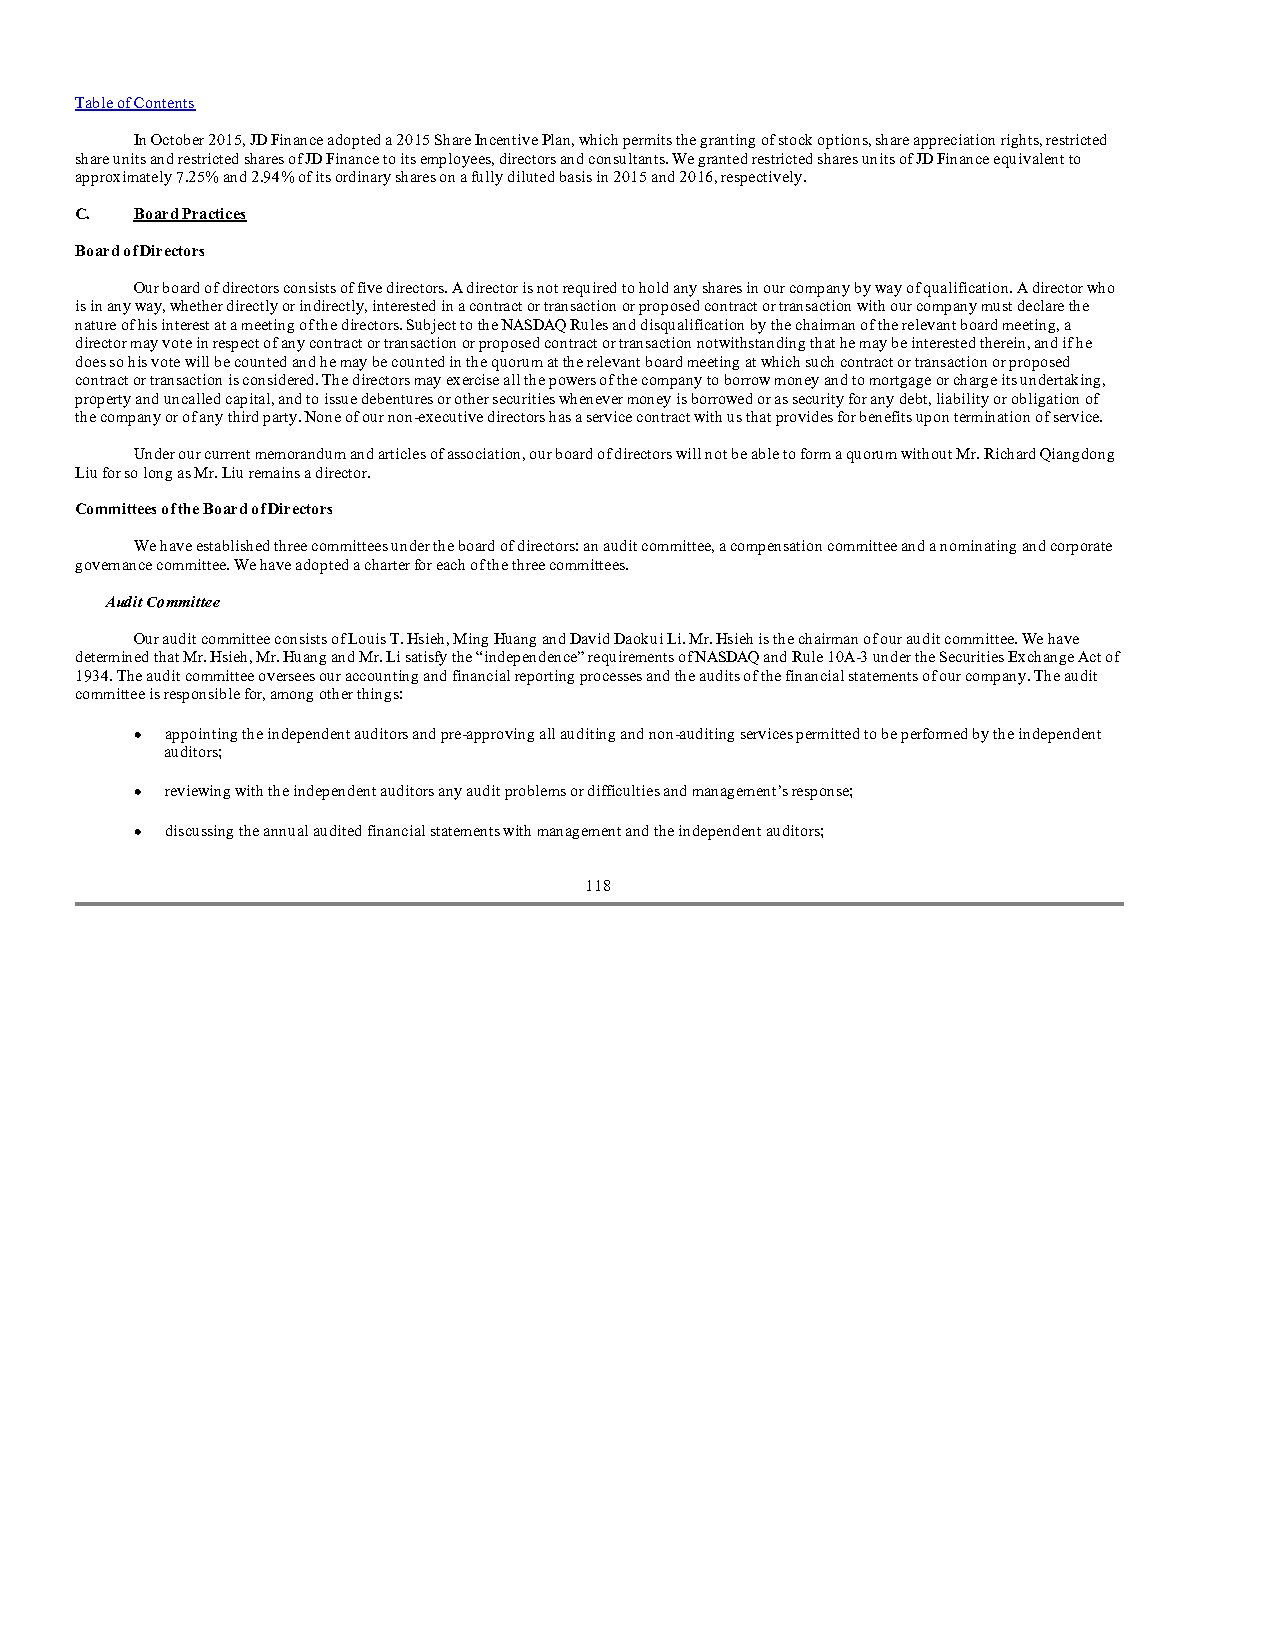
\includepdf[pages=-]{appendix.pdf} 
\newpage


%\section{Example Chapter}
%
%This is my text with an example Figure~\ref{fig:example} and example
%citation~\cite{StrunkWhite} or \textcite{Bringhurst1993}. And there is another
%\enquote{citation} which is located at the bottom\footcite{tagstore}.
%
%\myfig{TU_Graz_Logo}%% filename in figures folder
%  {width=0.1\textwidth,height=0.1\textheight}%% maximum width/height, aspect ratio will be kept
%  {Example figure.}%% caption
%  {}%% optional (short) caption for table of figures
%  {fig:example}%% label
%
%Now you are able to write your own document. Always keep in mind: it's
%the \emph{content} that matters, not the form. But good typography is
%able to deliver the content much better than information set with bad
%typography. This template allows you to focus on writing good content
%while the form is done by the template definitions.


%% vim:foldmethod=expr
%% vim:fde=getline(v\:lnum)=~'^%%%%\ .\\+'?'>1'\:'='
%%% Local Variables: 
%%% mode: latex
%%% mode: auto-fill
%%% mode: flyspell
%%% eval: (ispell-change-dictionary "en_US")
%%% TeX-master: "main"
%%% End: 
